\chapter{Experiment Simulation}
\label{ch:Simulation}

Simulated data, or Monte Carlo (MC), plays a very important role in the \nova~analyses. The FD only expects $O(10^2)$ events per year, not nearly enough statistics to fine tune things like selection cuts. Furthermore, it is important that actual parameter measurements use an independent sample of data from that used to train and tune an anlysis. MC solves both of these problems by being explicitly different from the real data and having only computer memory limit statistics.

The full simulation chain is very long and comprises multiple steps, which reduces complexity and provides more opportunity for validation. At every step, the information from previous pieces of the simulation chain are kept so it is always possible to reproduce future results and trace any errors that may occur. The simulation chain consists of two main components, simulation of the beam and the detector response. This chapter discusses both of these areas in more detail, and finishes with a discussion of packages designed to study and validate the results.

\section{Flux Simulation}

The first main simulation segment is the simulation of the NuMI beam, or the flux simulation. This section starts with the interaction of protons in the target and ends with experiment independent flux files full of neutrino rays that most importantly contain the flavor, direction, energy, and momentum of the neutrinos.

The flux simulation is performed using the FLUGG package, an interface between FLUKA \cite{ref:Fluka1, ref:Fluka2} and Geant4 \cite{ref:Geant41, ref:Geant42}. The version used for the analysis in this dissertation was FLUGG 2009.3, combining FLUKA2011 and Geant4 v4.9.6.p03(c). The FLUKA package is designed to simulate particle interactions and was used to simulate the proton interactions in the target. Geant4 is a toolkit for simulation of particles propagating through matter, and is used in this context to propagate the target interaction products through a detailed model of the NuMI beam line. This model of the beam includes all of the elements discussed in section \ref{sec:NuMI}, starting from the target hall all the way through the rock before the detector halls. The second focusing horn, a representative component of the geometry model, is shown in figure \ref{fig:GeomHorn}.
\begin{figure}[htb]
  \centering
  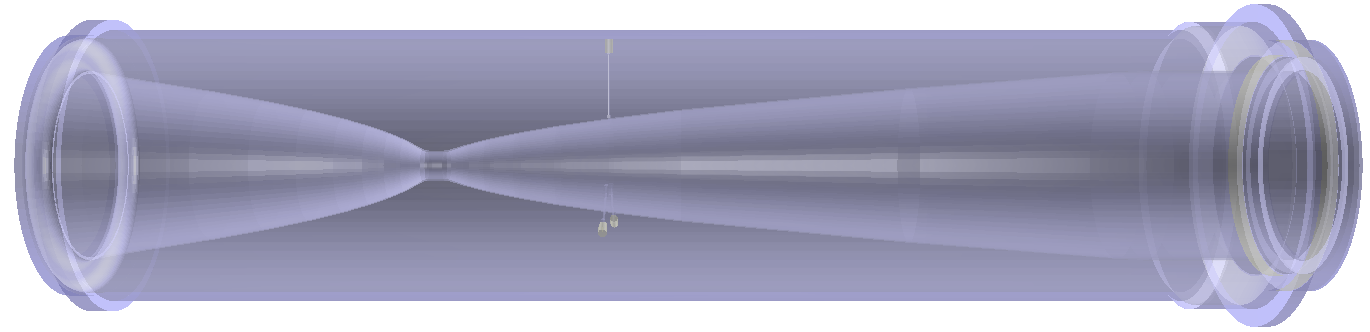
\includegraphics[width=0.9\textwidth]{figures/Horn2.png}
  \caption[Model of the Second Focusing Horn]{Visualization of the geometry used to model the second horn. This image was made during efforts to correctly position the three spider supports seen near the center of the schematic. Figure from \cite{ref:GeomNuMI}.}
  \label{fig:GeomHorn}
\end{figure}

\section{Detector Simulation}

\section{Validation}